\documentclass[12pt,a4paper]{scrartcl}

\usepackage[utf8]{inputenc}
\usepackage[T1]{fontenc}
\usepackage[ngerman]{babel}

\usepackage[pdftex]{graphicx}
\usepackage{latexsym}
\usepackage{amsmath,amssymb,amsthm}
\allowdisplaybreaks
\usepackage{dsfont}
\usepackage{pifont}
\usepackage{nicefrac}
\usepackage{textcomp}
\usepackage{enumitem}
\usepackage{lmodern}

% Abstand obere Blattkante zur Kopfzeile ist 2.54cm - 15mm
\setlength{\topmargin}{-15mm}	   
                  
\numberwithin{equation}{section} 

\newcommand{\C}{\mathbb{C}} % komplexe
\newcommand{\K}{\mathbb{K}} % komplexe
\newcommand{\R}{\mathbb{R}} % reelle
\newcommand{\Q}{\mathbb{Q}} % rationale
\newcommand{\Z}{\mathbb{Z}} % ganze
\newcommand{\N}{\mathbb{N}} % natuerliche
\newcommand{\PP}{\mathbb{P}} % Probability
\newcommand{\E}{\mathcal{E}} % big Epsilon

\numberwithin{equation}{section}%

\theoremstyle{definition}
\newtheorem{exmp}{Example}[section]
\newtheorem{theorem}{Theorem}[section]
\newtheorem{corollary}{Corollary}[theorem]
\newtheorem{lemma}[theorem]{Lemma}
\newtheorem{definition}[theorem]{Definition} 
\newtheorem{proposition}[theorem]{Proposition}

\newtheorem{thm}{Theorem}[section]%
\newtheorem{lem}[thm]{Lemma}%
\newtheorem{satz}[thm]{Satz}%
\newtheorem{prop}[thm]{Proposition}%
\newtheorem{algo}[thm]{Algorithmus}%

\newtheorem{cor}[thm]{Corollary}%
\theoremstyle{definition}
\newtheorem{dfn}[thm]{Definition}%
\newtheorem{rem}[thm]{Remark}%
\newtheorem{com}[thm]{Comment}
\newtheorem{exa}[thm]{Example}%
\newtheorem{bew}[thm]{Beweis}%


\begin{document}
	\pagestyle{empty}

\begin{titlepage}

	
\includegraphics[scale=0.45]{kit-logo.jpg} 
    \vspace*{2cm} 
\begin{center} \large 
    
   Masterthesis
    \vspace*{2cm}

    {\huge External DLA}\\
    \vspace*{2.5cm}

    Tillmann Tristan Bosch
    \vspace*{1.5cm}

    10. March 2020
    \vspace*{3.5cm}


    Supervisor: PD. Dr. Steffen Winter \\[1cm]
    Faculty of Mathematics\\[1cm]
	Karlsruhe Institute of Technology
\end{center}
\end{titlepage}

\newpage

\newpage
\phantom \\
\newpage

\tableofcontents %Inhaltsverzeichnis

 	\pagestyle{headings}

\setcounter{page}{1}
\section{Einleitung}
External DLA beschreibt einen stochastischen Prozess, welcher zumindest in ähnlicher Form in natürlichen Prozessen beobachtbar ist. Er ähnelt zum Beispiel der fraktalen Gestalt eines sich kreisförmig ausbreitenden Risses einer Glasscheibe, oder eines Risses eines Kristallfluids wie in LCD Displays in alten Autoradios (siehe Fotos). Er kann auch in Schneeflocken oder in elektrostatischen Anhaftungen an Metallen beobachtet werden. Die Formalisierung solcher Prozesse ist sehr aktuell und die sehr konstruktive Definition erlaubten bisher nur mühsame Folgerungen über Struktur und Verhalten des Prozesses. Wir werden uns Modelle auf $\mathbb{Z}^2$, sowie auf anderen Graphen, darunter auch fraktale Graphen, anschauen, und außerdem versuchen, eine Approximation der bisherigen Definition zu finden, die grundsätzlich handlicher ist und auf einfachere Weise zu Erkenntnissen führt. Wir werden außerdem diese Arbeit mit einigen Python Simulationen begleiten. Der Code ist frei verfügbar auf Github. \\
\\

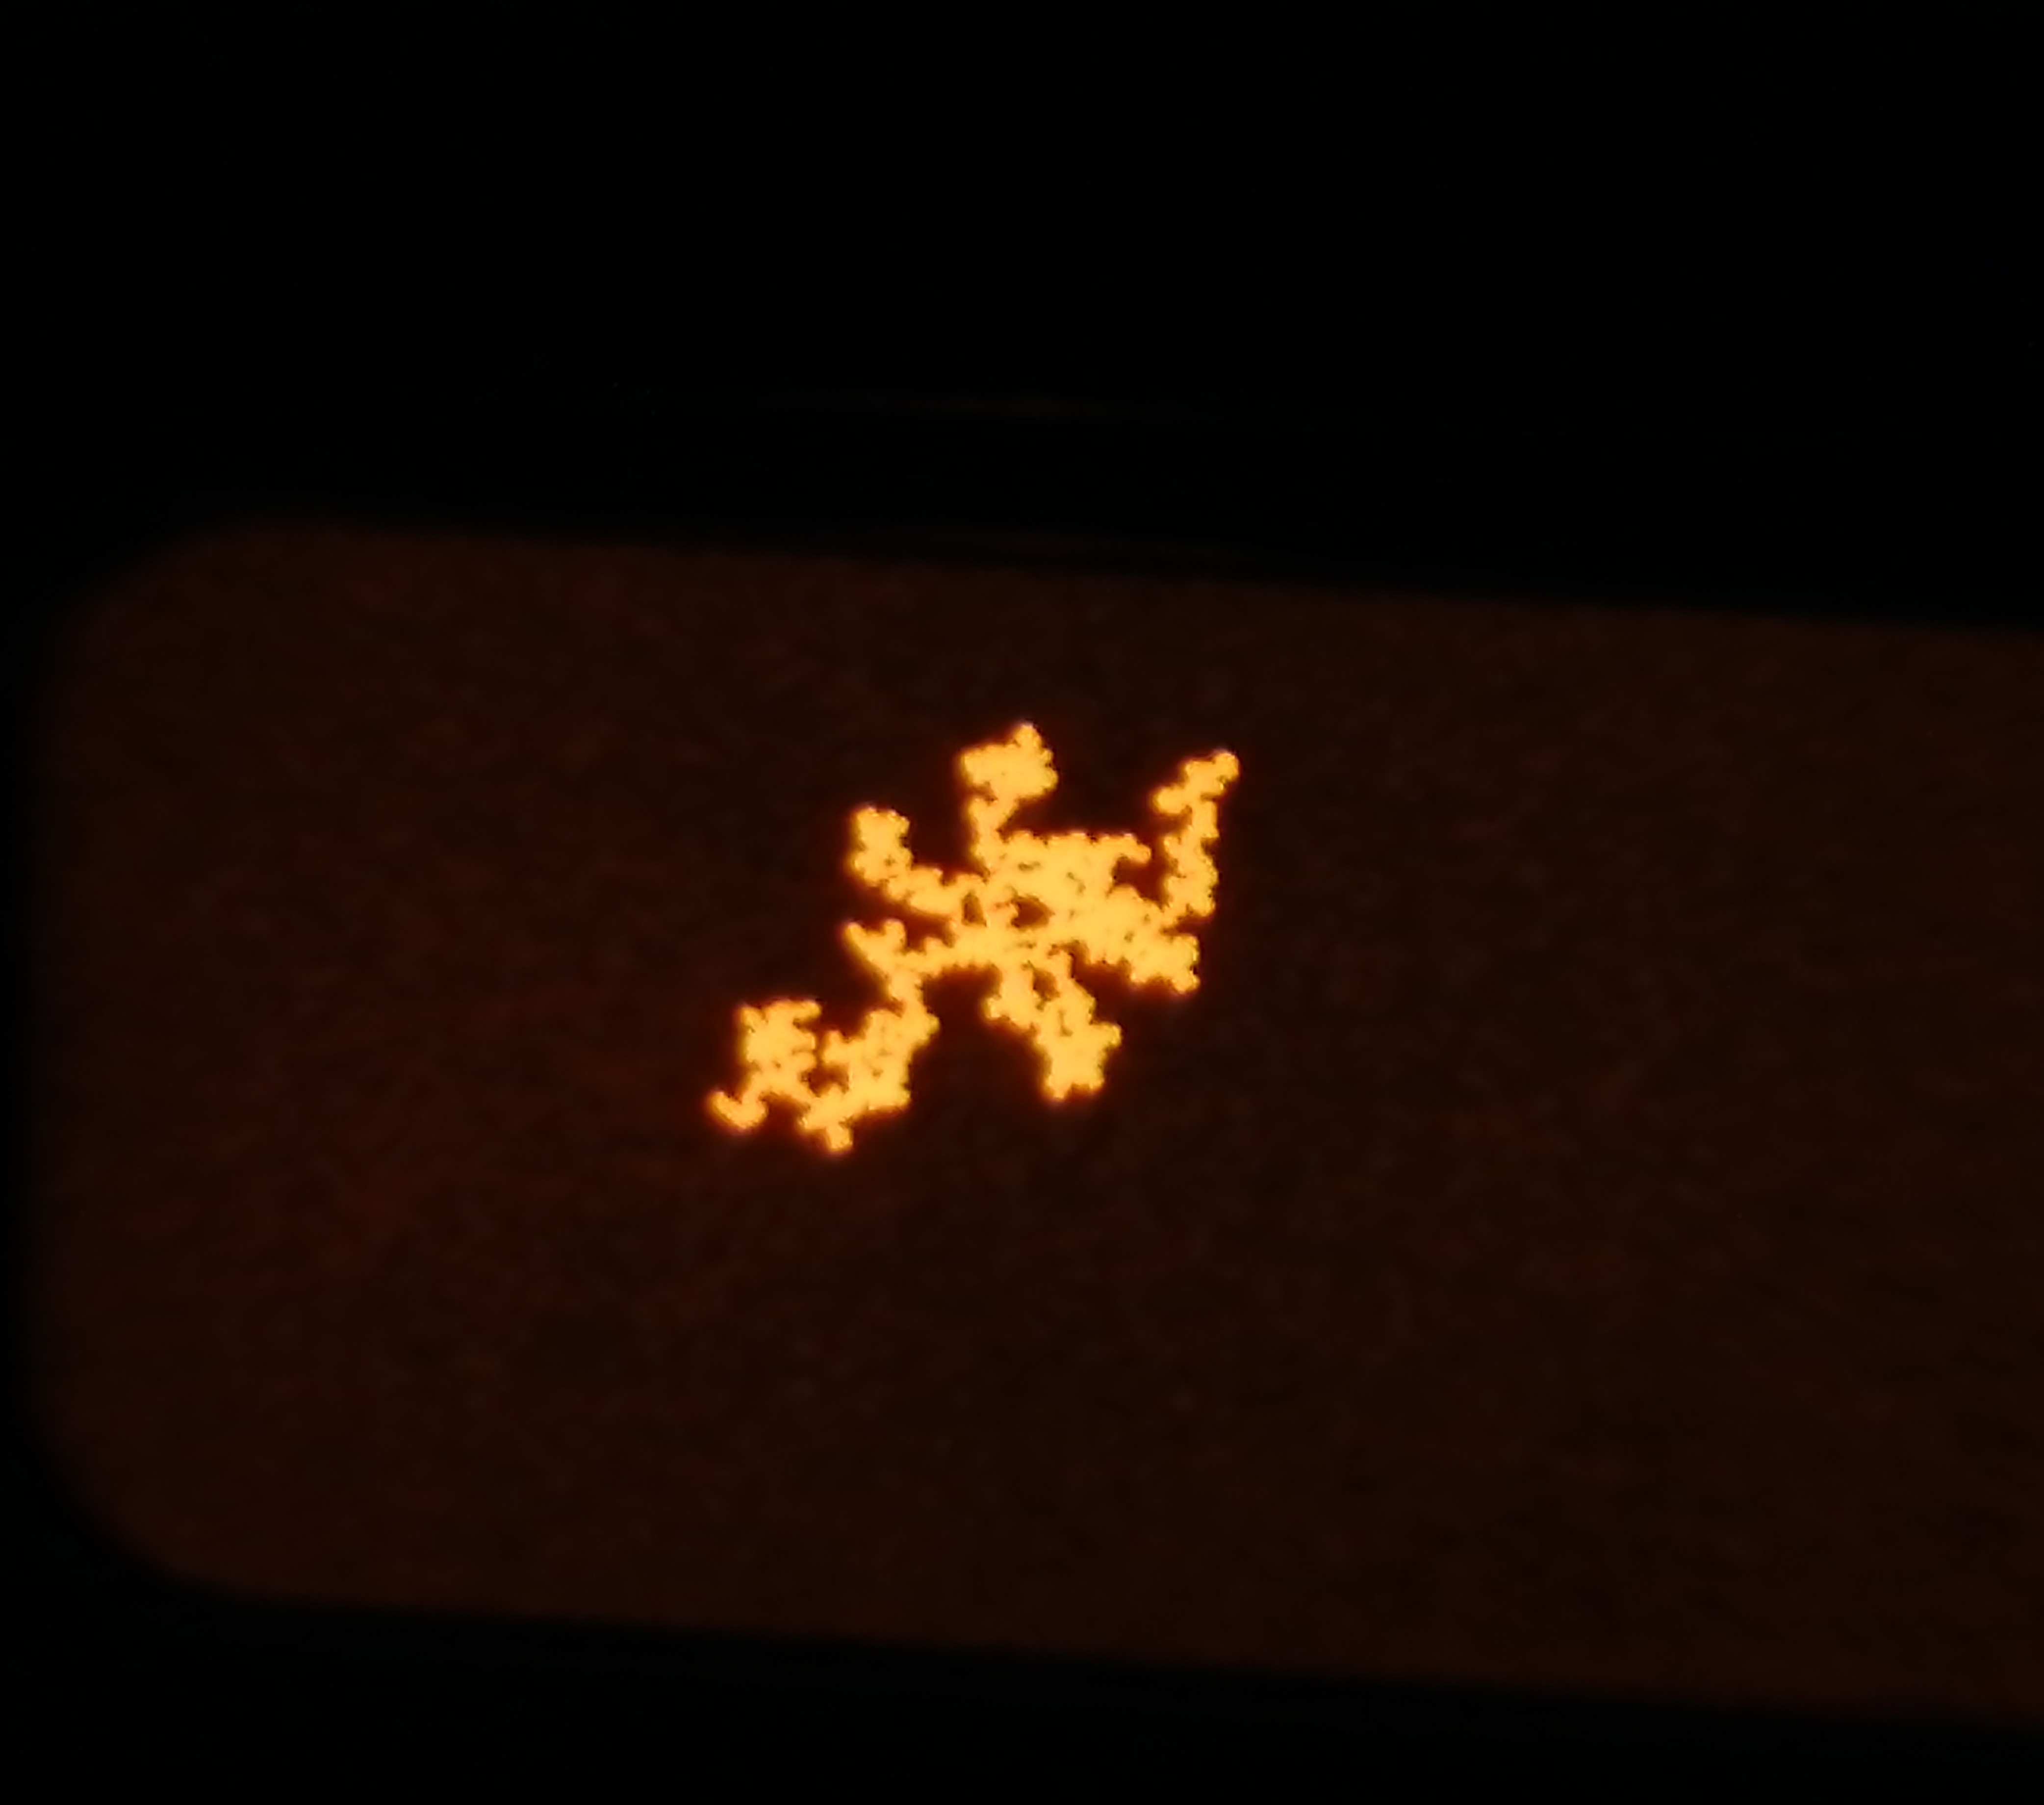
\includegraphics[scale=0.04]{display.jpg} 

\includegraphics[scale=0.091]{display2.jpg} 

\newpage


\section{Preliminaries} \label{prelim}

We prepare this script with the following preliminaries. \\
\\
$\boldsymbol{\mathit{Graphs}}.\quad$ In this paper we will be interested in the graph $(\mathbb{Z}^d, E)$ with the canonical graph structure, which is $x,y\in \mathbb{Z}^d$ form an edge (e.q. $(x,y)\in E$) if and only if $\exists ! i\in \{1,\dots, d\}$ such that $|x_i - y_i| = 1$ and $x_j = y_j$ for all $j\neq i$. For a point $x\in \mathbb{Z}^d$ its set of $\mathit{neighbours}$ is defined as $N(x) := \{y\in \mathbb{Z}^d\ |\ (x,y)\in E\}$ and the canonical graph structure as defined above basically means that $N(x) = \{x+re_i\ |\ r\in \{-1,1\}\text{ and } i\in \{1,\dots, d\}\}$, $e_i$ being the usual unit vectors of $\mathbb{Z}^d$. For a set $A\subset \mathbb{Z}^d$ the $\mathit{edgeset}\ \partial A$ of $A$ is defined as $\partial A := \{y\in \mathbb{Z}^d\ |\ \exists x\in A:\ (x,y)\in E\}$. From now on insted of $(\mathbb{Z}^d, E)$ we will write $\mathbb{Z}^d$. 
\\

\noindent $\boldsymbol{\mathit{Random\ Walks}}.\quad$ Let $(S_n)_n$ be a random walk on $G$ and denote $\mathbb{P}_x$ the probability measure of the random walk started at $x$. That means precisely 
\begin{align*}
	\mathbb{P}_x(A) := \mathbb{P}_{S_n}(A|S_0=x) = \mathbb{P}(S_n\in A|S_0=x)
\end{align*}
for any subset $A\subset G$. We define the $hitting\ time$ of A as 
\begin{align*}
	T(A) := \min \{n\geq 0\ |\ S_n\in A\},
\end{align*}
and for the special case $T(\{x\})=:T(x)$ for every $x\in G$. The $heat\ kernel$ of the random walk $S_n$ is defined to be 
\begin{align*}
	p_n(x,y):=\mathbb{P}_x(S_n=y)
\end{align*}
and following the $Green\ function$ as 
\begin{align*}
	G(x,y) := \sum_{n\geq 0} p_n(x,y).
\end{align*}
Similarily for a subset $A\subset G$ the $killed$ or $stopped\ Green\ function$ is defined as
\begin{align*}
	G_A(x,y) := \sum_{n\geq 0} \mathbb{P}_x(S_n=y, T(A) > n).
\end{align*} 


\newpage
\section{Incremental Aggregation}
In this paper we will look at stochastic processes on the set of finite subsets of $\mathbb{Z}^d$, where we start with a one point set at $(0,0)$ and incrementally add a point on the edgeset of the current cluster according to some distribution. What we get is a randomly, point-by-point growing connected cluster which here we will call $\mathit{Incremental\ Aggregation}$. Define 
\begin{align}
	\mathcal{P}_C := \{A\subset \mathbb{Z}^d\ |\ \text{A is finite and connected}\}, 
\end{align}
the set of finite and connected subsets of $\mathbb{Z}^d$. Furthermore we will be interested in distributions on those sets, so for $A\in \mathcal{P}_C$ we define 
\begin{align}
	\mathcal{D}_A:= \{\mu: \mathbb{Z}^d\to [0,1]\ |\ \mu(y) = 0, \forall y\notin A\ \text{and}\ \sum_{y\in A} y = 1 \}.
\end{align}
So every element in $\mathcal{D}_A$ naturally defines a distribution on the elements of $A$. Now we define incremental aggregation as follows.  

\begin{definition}
	Let $\mu=(\mu_A)_{A\in \mathcal{P}_C}$ be a family of distributions with $\mu_A\in \mathcal{D}_A$ for all $A\in \mathcal{P}_C$. $\mathit{Incremental\ Aggregation\ (with\ distribution\ \mu)}$ is a stochastic process $(\mathcal{E}_n)_{n\in{\mathbb{N}_0}}$ which evolves as follows. The process starts with one point $\mathcal{E}_0 = \{(0,0)\}$. Knowing the process $\mathcal{E}_n$ at time $n$, let $y_n$ be a random point on $\partial \mathcal{E}_n\in \mathcal{P}_C$ with distribution
	\begin{align}
		\mathbb{P}(y_n = y\ |\ \mathcal{E}_n) := \mu_{\partial \mathcal{E}_n}(y),\quad y\in \mathbb{Z}^d.
	\end{align}
	We then define $\mathcal{E}_{n+1} := \mathcal{E}_n \cup \{y_n\}$.
\end{definition} 

\begin{rem}
	
\end{rem}



\newpage

\newpage
\section{External DLA}

External DLA is a model of Incremental Aggregation as defined above using a very natural distribution, called the $\mathit{harmonic\ measure}$. 

\begin{definition} $\mathit{(Harmonic\ Measure)}$\\
	\\
	Remembering the definitions in \eqref{prelim}, especially the heat kernel $p_n(x,y):=\mathbb{P}_x(S_n=y)$ of a random walk, the $\mathit{hitting\ distribution}$ of elements in $A$ with $\mathit{hitting\ position}$ $S_{T(A)}$ is 
	\begin{align*}
	H_A(x,y) := p_{T(A)}(x,y),\quad y\in A, 
	\end{align*}
	and for the special case $x=o:=(0,0)$ we define
	\begin{align*}
	h_A(y) := H_A(o,y) = \mathbb{P}_o(S_{T(A)}=y),\quad y\in A.
	\end{align*}
	Thus, $h_A(y)$ is the probability of hitting $A$ for the first time at $y$ starting from $o$. $h_A$ is called the $\mathit{harmonic\ measure\ (from\ o)}$.
\end{definition}

\begin{lemma}
	harmonic measure := hearmonic measure from infinity. Why does this exist?
\end{lemma}

\begin{definition} $\mathit{(External\ Diffusion\ Limited\ Aggregate,\ External\ DLA)}$\\
	\\ Incremental Aggregation with the harmonic measure $h$ as its distribution we define here, and in literature is known as $\mathit{Exernal\ Diffusion\ Limited\ Aggregate}$, short $\mathit{External\ DLA}$.
\end{definition}

\begin{rem}
	contenu...
\end{rem}


\newpage


\section{Line Process}

In the following we will look at a process which is the approach of a simple approximation of external DLA on $\mathbb{Z}^2$. The idea is to let particles move on straight lines coming from infinity and add to the cluster when hitting it. Obviously in most cases particles cannot move completely straight on $\mathbb{Z}^2$. Therefore we will consider points in $\mathbb{Z}^2$ as the centers of unit squares and let the particles move on straight lines in the full plane $\mathbb{R}^2$. We consider the line hitting a point in $\mathbb{Z}^2$ if and only if it cuts its unit square as defined in the following. 

\begin{definition}
	Define 
	\begin{align}
		G_{sq} := \{[k - \frac{1}{2}, k + \frac{1}{2}) \times [l- \frac{1}{2}, l + \frac{1}{2}) \subset \mathbb{R}^2\ |\ k,l \in \mathbb{Z}\}, 
	\end{align} 
	note that $\mathbb{R}^2 = \bigcup_{s\in G_{sq}} s$ and $s_1\cap s_2 = \emptyset$ for all $s_1\neq s_2\in G_{sq}$. The canonical function
	\begin{align}
	sq: \mathbb{Z}^2 \to G_{sq},\quad (k,l)\to [k - \frac{1}{2}, k + \frac{1}{2}) \times [l- \frac{1}{2}, l + \frac{1}{2})
	\end{align}
	is bijective and intuitively identifies points in $\mathbb{Z}^2$ with squares in $\mathbb{R}^2$. In the following when using a point $p\in \mathbb{Z}^2$ it will reference the point in $\mathbb{Z}^2$ or the corresponding square in $\mathbb{R}^2$ respecting the context. This bijection also naturally defines a graph structure on $G_{sq}$, which is two squares $s_1, s_2\in G_{sq}$ form an edge if and only if $sq^{-1}(s_1)$ and $sq^{-1}(s_2)$ form an edge in $G$. We call $L\subset \mathbb{R}^2$ a $line$ if and only if there exist $a,b\in \mathbb{R}^2$ such that $L=\{a+tb\in \mathbb{R}^2\ |\ t\in \mathbb{R}\}$. For the following context we say a line $L$ $hits$ a point $p\in \mathbb{Z}^2$ if and only if $L\cap sq(p) \neq \emptyset$.
	
\end{definition}

BILD Linie durch squares "hitting"\\
Gradenmaß

\begin{definition} $\mathit{Line\ Hitting\ Distribution}$\\
	contenu...
\end{definition}

\begin{definition} $\mathit{Line\ Process}$\\
	contenu...
\end{definition}



\newpage


\section{Notizen}

diffusion in fractals: $d_f < d$ (space $\mathbb{Z}^d$)


\newpage

\begin{thebibliography}{Lam00}
\thispagestyle{empty}

\bibitem{Henze Skript}
N. Henze.
\emph{Maß und Wahrscheinlichkeitstheorie (Stochastik II)}.
Karlsruher Institut für Technologie, Karlsruhe, 2010

\end{thebibliography}

\newpage
  
\thispagestyle{empty}

\vspace*{8cm}


\section*{Erklärung}

Hiermit versichere ich, dass ich diese Arbeit selbständig verfasst und keine anderen als die angegebenen Quellen und Hilfsmittel benutzt, die wörtlich oder inhaltlich übernommenen Stellen als solche kenntlich gemacht und die Satzung des Karlsruher Instituts für Technologie zur Sicherung guter wissenschaftlicher Praxis in der jeweils gültigen Fassung beachtet habe. \\[2ex] 

\noindent
Karlsruhe, den 10. März 2020\\[5ex] 

\end{document}

